\documentclass[11pt,a4paper]{article}
\usepackage[margin=1in]{geometry}
\usepackage[T1]{fontenc}
\usepackage{times}
\usepackage{float}
\usepackage{caption}
\captionsetup{font=small,labelfont=bf}
\usepackage{amsmath,amssymb}
\usepackage{graphicx}
\usepackage{booktabs}
\usepackage{multirow}
\usepackage[hidelinks]{hyperref}
\usepackage{cite}
\usepackage{tikz}
\usetikzlibrary{positioning,arrows.meta}
\newcommand{\PROTRAND}{0.948}
\newcommand{\PROTSUBJ}{0.929}
\newcommand{\PROTLOCO}{0.912}
\newcommand{\PROTCARE}{0.860}
\newcommand{\PROTLAB}{0.932}
\newcommand{\VALCARE}{0.949}
\newcommand{\VALGAP}{8.9}
\newcommand{\ECELAB}{0.045}
\newcommand{\ECECARE}{0.089}
\newcommand{\RECPICKLAB}{0.86}
\newcommand{\RECPICKCARE}{0.68}
\newcommand{\PTDCARE}{30\,\%}
\newcommand{\NFDELTA}{$\Delta=-0.017$, $p_{\mathrm{Holm}}=0.278$}
\newcommand{\DUALDELTA}{$\Delta=+0.002$, $p_{\mathrm{Holm}}=1.000$}
\newcommand{\RESDELTA}{$\Delta=-0.003$, $p_{\mathrm{Holm}}=1.000$}
\newcommand{\DUALRES}{0.905 $\rightarrow$ 0.911}
\newcommand{\NFSVM}{0.538/0.565}
\newcommand{\ENSF}{0.922}
\newcommand{\ADADELTA}{$\Delta=+0.009$, $p_{\mathrm{Holm}}=0.087$}
\newcommand{\TENTDELTA}{$\Delta=+0.010$, $p_{\mathrm{Holm}}=0.003$}
\newcommand{\AUGDELTA}{$\Delta=+0.011$, $p_{\mathrm{Holm}}=1.000$}
\newcommand{\AUGADADELTA}{$\Delta=+0.017$, $p_{\mathrm{Holm}}=0.010$}
\newcommand{\KINDELTA}{$\Delta=+0.003$, $p_{\mathrm{Holm}}=1.000$}
\newcommand{\TRACKDELTA}{$\Delta=-0.007$, $p_{\mathrm{Holm}}=1.000$}
\newcommand{\INDELTA}{$\Delta=+0.013$, $p_{\mathrm{Holm}}=0.256$}
\newcommand{\MOBDELTA}{$\Delta=-0.026$, $p_{\mathrm{Holm}}=0.002$}
\newcommand{\HANNDELTA}{$\Delta=-0.010$, $p_{\mathrm{Holm}}=1.000$}
\newcommand{\AUGADAF}{0.925}
\newcommand{\AUGADACARE}{0.870}
\newcommand{\TENTF}{0.922}
\newcommand{\TENTCARE}{0.866}
\newcommand{\ADAF}{0.921}
\newcommand{\INF}{0.921}
\newcommand{\DUALF}{0.914}
\newcommand{\BASEF}{0.912}
\newcommand{\BASESEEDS}{10}
\newcommand{\ENSSRC}{0.922}
\newcommand{\ENSADA}{0.926}
\newcommand{\LFSRC}{0.924}
\newcommand{\LFADA}{0.934}
\newcommand{\DUALVSENS}{-0.009}
\newcommand{\DUALVSENSP}{0.001}
\newcommand{\LFVSENS}{+0.006}
\newcommand{\LFVSENSP}{0.028}


\emergencystretch=3em
\begin{document}


\title{Moving Micro-Doppler Activity Recognition to New Sites: A Leave-One-Campaign-Out Study of Low-Cost Remedies}
\author{Abdul Mannaan Sayyad\\ \normalsize Department of Computer Science and Engineering, VIT-AP University, Guntur, India\\ \normalsize \texttt{sd.abdulmannaan.31@gmail.com}}
\date{}


\maketitle

\begin{abstract}
Radar micro-Doppler classifiers of daily activities are usually evaluated with splits that share people and rooms between training and test. We evaluate a 5.8\,GHz FMCW activity classifier under leave-one-campaign-out (LOCO) testing on a public seven-campaign dataset that includes two care sites with older adults. Macro-F1 drops from \PROTRAND{} with random splits to \PROTLOCO{} under LOCO and to \PROTCARE{} on the care sites, where calibration error doubles. We then test low-cost remedies with paired statistics over 5--10 seeds: target-tracking range gates, CFAR-style noise-floor referencing, a dual-reference input, augmentation, ImageNet pre-training, label-free test-time adaptation (AdaBN, TENT) and enrollment of up to three labelled residents. The best combinations gain 1--2 points overall, but none narrows the laboratory-to-care-site gap of about seven points. The residual errors (pick-up vs.\ drinking) are consistent with cohort-level kinematic differences rather than site or sensor effects.
\end{abstract}

\noindent\textbf{Keywords:} micro-Doppler, FMCW radar, human activity recognition, domain shift, test-time adaptation, assisted living

\section{Introduction}
Radar is an attractive sensor for monitoring daily activities of older adults. It needs no contact, works in the dark and records no images~\cite{fioranelli2019health,shah2019review}. Micro-Doppler classifiers routinely report accuracies above 90\,\%~\cite{gurbuz2019spm,li2019survey}. However, in most evaluations the test recordings come from the same rooms, sessions and often the same people as the training data. Deployment is different: a model trained on earlier collections is installed in a \emph{new} room, with \emph{new} residents and a slightly different set-up. Whether reported accuracy survives that move is a practical question for radar-based assisted living. Answering it requires a protocol that holds out whole campaigns.

The radar front-end offers obvious remedies that need no new data. The range cells that are integrated into the spectrogram can follow the target. The image intensity can be referenced to the sensor noise floor instead of the strongest return, as a CFAR detector would~\cite{rohling1983cfar}. On the learning side, BatchNorm statistics can be re-estimated on unlabeled data from the new site~\cite{li2018adabn}. These remedies cost little, but on real cross-site micro-Doppler data they have not been compared with each other under one controlled protocol.

This paper studies them on the public Glasgow 5.8\,GHz FMCW dataset~\cite{gla848}. Its seven campaigns include two collected with older adults outside the laboratory. Our contributions are:
\begin{itemize}
\item a leakage-aware evaluation (one sample per recording, a duration-neutral 5\,s window, person identity across campaigns, a range gate defined in metres to handle a 100\,MHz subset) that quantifies the random $\rightarrow$ subject $\rightarrow$ LOCO decline with paired statistics;
\item a controlled comparison of radar front-end remedies (target tracking, maximum- vs.\ noise-floor referencing, range windowing, a dual-reference input), augmentation, pre-training, label-free test-time adaptation and few-person site enrollment, including the negative results and their physical explanation;
\item an error analysis showing that the residual cross-site gap is concentrated in the care-site cohorts (mostly older adults) and in kinematically similar actions, with source validation overstating care-site performance by \VALGAP{} points.
\end{itemize}
Code, configurations and all per-fold results are released.

\section{Related Work}
Micro-Doppler classification of human motion rests on the time-varying Doppler of body parts~\cite{chen2006microdoppler}. Early systems used hand-crafted features with SVMs~\cite{kim2009svm}. CNNs on spectrograms~\cite{kim2016dcnn,seyfioglu2018cae} and recurrent models~\cite{shrestha2020bilstm} followed; see the surveys~\cite{gurbuz2019spm,li2019survey}. The Glasgow dataset used here underlies the Human Activity Radar Challenge~\cite{yang2023challenge}. Shah et al.~\cite{shah2022portability} studied data portability across nine locations, including care homes. They pooled all locations and used repeated random 70/30 splits, so the same people and rooms appear on both sides of the split.

Robustness has mostly been studied with \emph{synthetic} perturbations. Zhou et al.~\cite{zhou2024corruption} benchmark temporal, Doppler and intensity corruptions; denoising against added white noise is studied in~\cite{nguyen2024noise}. Representation choices (range-time, range-Doppler, STFT, SPWVD) have been compared under within-dataset splits~\cite{ayaz2025sp,ayaz2026bench}. For real shifts, domain adaptation has been applied from simulated to measured data~\cite{li2020uda}, across mmWave environments with feature fusion and distillation~\cite{li2025crossenv}, and in source-free form~\cite{liu2024sfda,si2025sfda}. These methods train additional networks on target data. A preprint on FMCW people counting~\cite{tanaka2025crossenv} found that simple amplitude preprocessing recovered much of the cross-room loss. We ask the analogous question for micro-Doppler activity recognition: how far do low-cost remedies go, from the front-end intensity reference to label-free BatchNorm adaptation~\cite{li2018adabn,wang2021tent}?

\section{Signal Processing and Method}\label{sec:method}
\begin{figure}[t]
\centering
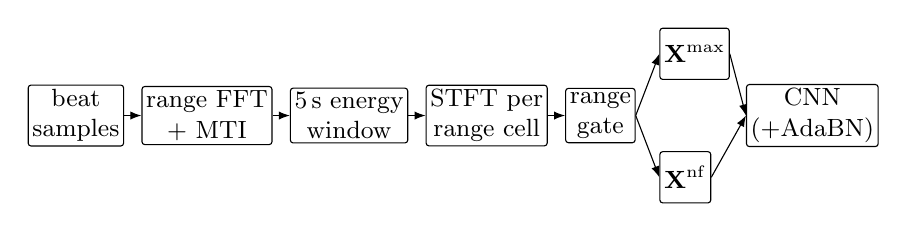
\begin{tikzpicture}[scale=1.0, transform shape, node distance=2.2mm, every node/.style={font=\small, align=center},
  blk/.style={draw, rounded corners=1pt, minimum height=6.5mm, inner sep=1.5pt, fill=white},
  arr/.style={-{Latex[length=1.4mm]}, thin}]
\node[blk] (adc) {beat\\ samples};
\node[blk, right=of adc] (rfft) {range FFT\\ + MTI};
\node[blk, right=of rfft] (win) {5\,s energy\\ window};
\node[blk, right=of win] (stft) {STFT per\\ range cell};
\node[blk, right=of stft] (gate) {range\\ gate};
\node[blk, above right=1.0mm and 3mm of gate] (max) {$\mathbf{X}^{\max}$};
\node[blk, below right=1.0mm and 3mm of gate] (nf) {$\mathbf{X}^{\mathrm{nf}}$};
\node[blk, right=14mm of gate] (cnn) {CNN\\ (+AdaBN)};
\draw[arr] (adc)--(rfft); \draw[arr] (rfft)--(win); \draw[arr] (win)--(stft); \draw[arr] (stft)--(gate);
\draw[arr] (gate.east)--(max.west); \draw[arr] (gate.east)--(nf.west);
\draw[arr] (max.east)--(cnn.west); \draw[arr] (nf.east)--(cnn.west);
\end{tikzpicture}
\caption{Processing chain. The dual-reference input stacks a maximum-referenced and a noise-floor-referenced micro-Doppler image as two channels.}
\label{fig:chain}
\end{figure}

\subsection{Range compression, clutter suppression and windowing}
Let $s_m[n]$, $n=0,\dots,N-1$, be the complex beat signal of chirp $m$ ($N=128$, chirp period $T_c=1$\,ms). The range profile is
$z_m[r]=\sum_{n} s_m[n]\,e^{-j2\pi nr/N}$, kept for the positive-beat bins $r=1,\dots,48$. With sweep bandwidth $B$, bin $r$ lies at range $R_r = r\,\Delta R$, $\Delta R=c/(2B)$. Static clutter is removed by a fourth-order Butterworth high-pass filter along slow time $m$ (cut-off 3.75\,Hz), as in the dataset's reference code. Walking recordings last 10\,s and the other activities 5\,s. To stop the classifier from learning duration, every recording is cut to the 5\,s window with maximum post-MTI energy $\sum_r |z_m[r]|^2$. This choice does not use the label.

\subsection{Micro-Doppler spectrogram and range gating}
For each range cell a short-time Fourier transform with a 200\,ms Hann window $w$, 20\,ms hop and 256-point FFT gives
\begin{equation}
P_r(f,t)=\Big|\sum_{m} z_{m}[r]\,w[m-tH]\,e^{-j2\pi f m T_c}\Big|^2 .
\end{equation}
The 128 Doppler bins in $|f|\le 250$\,Hz ($|v|\le 6.46$\,m/s at $\lambda=5.17$\,cm) are retained. A range gate $\mathcal{G}(t)$ forms $S(f,t)=\sum_{r\in\mathcal{G}(t)}P_r(f,t)$. The \emph{fixed} gate sums $3.75\le R_r\le 11.25$\,m (bins 10--30 at $B=400$\,MHz, as in the reference code), converted with each file's own $B$. The \emph{tracking} gate follows the mover: $r^\star(t)=\arg\max_r \sum_{|f|>f_0}P_r(f,t)$, median-filtered over 9 frames, and $\mathcal{G}(t)=\{r: |r-r^\star(t)|\Delta R\le 1.5\,\text{m}\}$. The time axis is average-pooled to 128 frames.

\subsection{Two intensity references}
With $L(f,t)=10\log_{10}S(f,t)$, the conventional \emph{maximum-referenced} image clips a dynamic range $D=40$\,dB below the peak:
\begin{equation}
X^{\max}=\tfrac{1}{D}\,\mathrm{clip}\big(L-\max_{f,t}L+D,\;0,\;D\big).
\end{equation}
It is invariant to receiver gain and path loss. However, the visible extent of weak limb returns depends on how far the strongest scatterer (usually the torso) rises above the floor. The \emph{noise-referenced} image instead measures each cell against a per-Doppler-bin floor estimated by an ordered statistic along slow time, as in OS-CFAR~\cite{rohling1983cfar}:
\begin{equation}
X^{\mathrm{nf}}=\tfrac{1}{D}\,\mathrm{clip}\big(L-\hat N(f)-\alpha,\;0,\;D\big),
\end{equation}
where $\hat N(f)=Q_{0.2}\{L(f,t)\}_t$ is the 20th percentile over time, with threshold margin $\alpha=6$\,dB. $X^{\mathrm{nf}}$ is a per-cell SNR map. It also removes Doppler-dependent residues of the MTI response. The proposed \emph{dual-reference} input is the two-channel image $[X^{\max}_{\text{fixed}},\,X^{\mathrm{nf}}_{\text{track}}]\in[0,1]^{2\times128\times128}$. The two channels see the same echo through different normalisations, and the classifier can weigh them per feature. The input costs one extra percentile per Doppler bin.

\subsection{Label-free test-time adaptation}
AdaBN~\cite{li2018adabn} replaces each BatchNorm layer's running mean and variance with statistics accumulated over the unlabeled recordings of the deployment campaign, without changing any weight. TENT~\cite{wang2021tent} additionally adapts the BatchNorm affine parameters by minimising prediction entropy on those recordings (one pass, Adam, lr $10^{-3}$). Both need no labels and suit a radar installed in a new room. Target batches are drawn in random order, because class-sorted batches bias the estimated statistics.

\section{Experimental Setup}\label{sec:setup}
\subsection{Data}
We use the public Glasgow \emph{Radar signatures of human activities} dataset~\cite{gla848} (CC BY 4.0). It was recorded with an Ancortek FMCW radar at 5.8\,GHz ($T_c=1$\,ms, 128 samples per chirp, Yagi antennas). The data come from seven campaigns: five in university rooms (Dec17, Mar17, Jun17, Jul18, Feb19) and two at sites with older participants (NG-H, care housing, ages 24--88; WC, an Age UK day centre). We use the five activities recorded in every campaign (walk, sit down, stand up, pick up an object, drink), one sample per recording. This gives 1656 recordings from 106 person-campaigns; three files whose name codes disagree were excluded. Two properties of the data matter for evaluation. First, subject IDs are re-used across campaigns, so identity is (campaign, ID). Second, 60 WC files use $B=100$\,MHz ($\Delta R=1.5$\,m) instead of 400\,MHz; this is visible only in the file headers. Fig.~\ref{fig:range} shows that subjects stood closer to the radar at the care sites. At NG-H only 14\,\% of the moving energy falls inside the fixed range gate, against 75--93\,\% in the lab campaigns.

\begin{figure}[t]
\centering
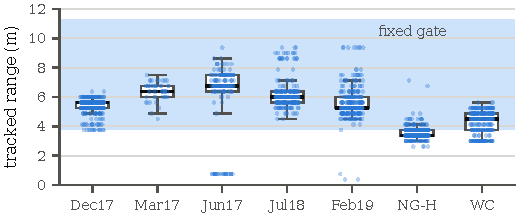
\includegraphics[width=0.62\linewidth]{figures/range_by_campaign.pdf}
\caption{Median tracked target range per recording and campaign. The shaded band is the fixed range gate of the reference processing.}
\label{fig:range}
\end{figure}

\subsection{Protocols}
\emph{Random}: stratified 5-fold over recordings, so the same people and rooms appear in training and test. \emph{Subject}: 5-fold grouped by person. \emph{LOCO}: leave-one-campaign-out, seven folds; the test campaign is a new site, cohort and session. In every protocol, 15\,\% of the training \emph{persons} form a validation set used for epoch selection. The test fold is evaluated once. AdaBN sees only the unlabeled test-campaign inputs.

\subsection{Models and training}
\emph{LightCNN} (four double-conv blocks, 16--128 channels, global pooling, 0.29\,M parameters), ResNet-18~\cite{he2016resnet} (11.2\,M) and MobileNetV2~\cite{sandler2018mobilenetv2} (2.2\,M) are trained from scratch with single- or two-channel stems. An ImageNet-pretrained ResNet-18, whose RGB stem is collapsed to the input channels, is also fine-tuned. As a classical baseline, SVM and random-forest classifiers use moments of the Doppler centroid, bandwidth and envelopes, the feature family of~\cite{shah2022portability}. Training uses AdamW (lr $10^{-3}$, weight decay $10^{-4}$), a one-cycle schedule, 40 epochs, batch size 32, class-balanced cross-entropy and fp16 autocast. Every condition uses five seeds (ten for the baseline and the dual-reference input). All networks were trained on one RTX\,4090. Controls are generic augmentation (time shift, intensity scale and offset, noise, time masking) and a radar-kinematic augmentation (velocity scaling $\times[1.3^{-1},1.3]$, tempo scaling $\times[1.25^{-1},1.25]$, dynamic range reduced to 20--40\,dB).

\subsection{Metrics and statistics}
The primary metric is macro-F1 on the held-out fold, averaged over folds and then over seeds. We also report accuracy, expected calibration error (ECE, 15 bins)~\cite{guo2017calibration} and per-campaign scores. Conditions are compared on paired (campaign, seed) scores (35 pairs; 70 for the ten-seed comparison) with two-sided Wilcoxon signed-rank tests, Holm-corrected over all 86 comparisons. Because seeds share folds, we base inference on 95\,\% confidence intervals from a cluster bootstrap over campaigns.

\section{Results and Discussion}\label{sec:results}
\begin{table}[t]
\centering
\caption{Macro-F1 under the three protocols (mean over five seeds; s.d.\ in units of $10^{-3}$ in parentheses). LOCO is also split into laboratory and care-site test campaigns.}
\label{tab:protocol}
\setlength{\tabcolsep}{2.5pt}
\footnotesize
\begin{tabular}{lccccc}
\toprule
 & & & & \multicolumn{2}{c}{LOCO split} \\
Model & Random & Subject & LOCO & lab & care \\
\midrule
SVM (features) & 0.860\,(3) & 0.850\,(2) & 0.818\,(6) & 0.827 & 0.797 \\
RF (features) & 0.860\,(4) & 0.846\,(7) & 0.832\,(5) & 0.854 & 0.777 \\
LightCNN & 0.948\,(5) & 0.929\,(4) & 0.912\,(8) & 0.932 & 0.860 \\
LightCNN, dual-ref. & 0.947\,(5) & 0.925\,(6) & 0.914\,(8) & 0.933 & 0.865 \\
\bottomrule
\end{tabular}
\end{table}
\begin{table}[t]
\centering
\caption{LOCO macro-F1 of each intervention (LightCNN unless stated; five seeds). $\Delta$: paired difference to the baseline with 95\,\% campaign-bootstrap CI; $p$: Holm-corrected Wilcoxon test over 35 (campaign, seed) pairs.}
\label{tab:interventions}
\setlength{\tabcolsep}{1.8pt}
\scriptsize
\begin{tabular}{lccccc}
\toprule
Condition & F1 & $\Delta$ [95\,\% CI] & $p$ & care & ECE \\
\midrule
\multicolumn{6}{l}{\emph{Reference}} \\
\quad fixed gate, max-ref. (baseline) & 0.912 & -- & -- & 0.860 & 0.057 \\
\multicolumn{6}{l}{\emph{Front-end}} \\
\quad tracking gate, max-ref. & 0.901 & -.007 [-.026,+.006] & 1.000 & 0.854 & 0.063 \\
\quad all range cells, max-ref. & 0.898 & -.010 [-.031,+.002] & 1.000 & 0.853 & 0.070 \\
\quad fixed gate, z-score & 0.907 & -.002 [-.019,+.019] & 1.000 & 0.846 & 0.062 \\
\quad fixed gate, noise-ref. ($\alpha$=6) & 0.902 & -.006 [-.019,+.007] & 1.000 & 0.838 & 0.059 \\
\quad tracking, noise-ref. $\alpha$=0 & 0.890 & -.018 [-.038,+.001] & 0.664 & 0.842 & 0.061 \\
\quad tracking, noise-ref. $\alpha$=6 & 0.891 & -.017 [-.035,+.003] & 0.278 & 0.827 & 0.063 \\
\quad tracking, noise-ref. $\alpha$=12 & 0.892 & -.016 [-.031,-.004] & 0.194 & 0.842 & 0.061 \\
\quad tracking, scalar noise-ref. & 0.893 & -.015 [-.035,+.003] & 1.000 & 0.848 & 0.064 \\
\multicolumn{6}{l}{\emph{Dual-reference input}} \\
\quad max + noise-ref. ($\alpha$=6) & 0.914 & +.002 [-.007,+.011] & 1.000 & 0.865 & 0.059 \\
\quad max + noise-ref. ($\alpha$=0) & 0.908 & +.000 [-.015,+.016] & 1.000 & 0.862 & 0.057 \\
\quad max + noise-ref. ($\alpha$=12) & 0.912 & +.004 [-.004,+.012] & 1.000 & 0.861 & 0.060 \\
\quad max + fixed-gate noise-ref. & 0.907 & -.001 [-.020,+.015] & 1.000 & 0.853 & 0.059 \\
\quad max + tracking max-ref. & 0.900 & -.008 [-.034,+.012] & 1.000 & 0.849 & 0.063 \\
\multicolumn{6}{l}{\emph{Training / adaptation}} \\
\quad generic augmentation & 0.919 & +.011 [-.000,+.022] & 1.000 & 0.862 & 0.054 \\
\quad kinematic augmentation & 0.911 & +.003 [-.010,+.016] & 1.000 & 0.857 & 0.057 \\
\quad AdaBN & 0.921 & +.009 [+.003,+.017] & 0.087 & 0.866 & 0.057 \\
\quad TENT & 0.922 & +.010 [+.004,+.017] & 0.003 & 0.866 & 0.057 \\
\quad dual-ref. + AdaBN & 0.922 & +.010 [-.001,+.021] & 0.324 & 0.871 & 0.056 \\
\multicolumn{6}{l}{\emph{Architecture}} \\
\quad ResNet-18 & 0.905 & -.003 [-.012,+.005] & 1.000 & 0.843 & 0.073 \\
\quad ResNet-18, dual-ref. & 0.911 & +.003 [-.003,+.009] & 1.000 & 0.850 & 0.073 \\
\quad MobileNetV2 & 0.882 & -.026 [-.038,-.017] & 0.002 & 0.835 & 0.090 \\
\quad MobileNetV2, dual-ref. & 0.879 & -.029 [-.044,-.012] & 0.007 & 0.826 & 0.090 \\
\quad ResNet-18, ImageNet init. & 0.921 & +.013 [+.002,+.024] & 0.256 & 0.867 & 0.063 \\
\quad ResNet-18 IN-init., dual-ref. & 0.916 & +.008 [-.003,+.019] & 1.000 & 0.865 & 0.066 \\
\bottomrule
\end{tabular}
\end{table}

\subsection{How much do protocols inflate performance?}
Table~\ref{tab:protocol} shows a monotone decline for every model as the protocol removes shared information. For LightCNN, macro-F1 falls from \PROTRAND{} (random) to \PROTSUBJ{} (subject-disjoint) and \PROTLOCO{} (LOCO, \BASESEEDS{} seeds). The decline is concentrated on the two care-site campaigns (\PROTCARE{}), while the five laboratory campaigns stay at \PROTLAB{}. Source validation is a poor proxy for deployment: the mean validation score of the care-site folds (\VALCARE{}) overstates their test score by \VALGAP{} points. The same folds show roughly double the calibration error (ECE \ECELAB{} vs.\ \ECECARE{}). The CNN outperforms the hand-crafted SVM/RF baselines by 8--10 points under every protocol.

\subsection{Do low-cost remedies close the gap?}
\emph{Front-end.} No front-end change improves on the reference processing (Table~\ref{tab:interventions}). Range tracking is neutral (\TRACKDELTA{}), and so is a Hann range window (\HANNDELTA{}). Even at NG-H the fixed gate still collects part of the moving energy (14\,\% on average), and maximum referencing removes the resulting level difference. Noise-floor referencing is worse in six of seven campaigns (\NFDELTA{}). Fig.~\ref{fig:examples} shows why: referencing to the floor exposes campaign-specific broadband stripes and interference lines that maximum referencing hides below its 40\,dB window. The same structure corrupts centroid and bandwidth features, so SVM/RF on noise-referenced images drop to \NFSVM{}. Stacking both references as two input channels does not help (\DUALDELTA{}; ten seeds) and is worse than a plain two-seed ensemble of the baseline (\DUALVSENS{}, $p$=\DUALVSENSP{}).

\emph{Learning.} Label-free test-time adaptation gives small, consistent gains: TENT \TENTDELTA{}, AdaBN \ADADELTA{}. Generic augmentation combined with AdaBN is the best LightCNN configuration (\AUGADAF{}, \AUGADADELTA{}), while kinematic augmentation is neutral (\KINDELTA{}). Capacity alone does not help: a scratch ResNet-18 matches LightCNN (\RESDELTA{}) and MobileNetV2 is worse (\MOBDELTA{}). ImageNet pre-training gives the largest single-model gain (\INF{}, \INDELTA{}), but it is not significant after correction.

\emph{The care-site gap persists.} Every remedy that raises the overall score raises the laboratory and care-site campaigns together. The best configuration reaches \AUGADACARE{} at the care sites against \PROTCARE{} for the baseline, while its laboratory score rises by a similar amount, so the gap stays at about seven points (Fig.~\ref{fig:percamp}). Two further observations come with caveats. First, the ResNet-18 shows a small, non-significant gain from the dual input (\DUALRES{}). Second, late fusion of separately trained max- and noise-referenced models (\LFADA{} with AdaBN) slightly exceeds a same-size seed ensemble (\LFVSENS{}, $p$=\LFVSENSP{}, uncorrected). The second idea was formed after a pilot that saw test scores, so we treat both as hypotheses. Effects of this size are also comparable to the $\approx$1-point difference we measured between re-runs of identical code on two GPU platforms.

\begin{figure}[t]
\centering
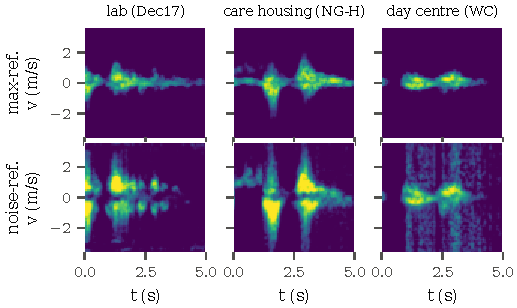
\includegraphics[width=0.62\linewidth]{figures/examples.pdf}
\caption{\emph{Pick up} recordings from three campaigns. Top: maximum-referenced input (40\,dB). Bottom: noise-referenced input, which also shows campaign-specific broadband interference (right).}
\label{fig:examples}
\end{figure}

\begin{figure}[t]
\centering
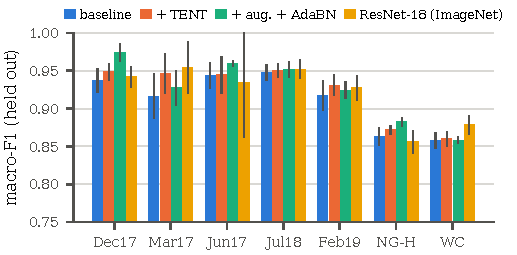
\includegraphics[width=0.62\linewidth]{figures/per_campaign.pdf}
\caption{Held-out macro-F1 per campaign (mean $\pm$ s.d.\ over seeds). The care sites NG-H and WC remain about seven points below the laboratory campaigns under every remedy.}
\label{fig:percamp}
\end{figure}

\subsection{Error analysis and site enrollment}
At the care sites, recall of \emph{pick up} falls from \RECPICKLAB{} to \RECPICKCARE{}, and \PTDCARE{} of pick-ups are labelled \emph{drink}. Older participants performed both actions with similar trunk and arm Doppler. If the residual gap stems from individual kinematics rather than from the room, a few labelled people from the new site should not fix it. Table~\ref{tab:enroll} is consistent with this. Fine-tuning with all recordings of one to three enrolled persons (recipe chosen by nested selection on a training campaign) does not improve F1 on the remaining residents beyond unlabeled AdaBN. In this dataset the gap therefore appears to be person- and cohort-level rather than site-level, and more diverse training cohorts are likely required.

\begin{table}[t]
\centering
\caption{Site enrollment (LOCO, LightCNN): macro-F1 on the non-enrolled persons of the held-out campaign (Mar17 excluded). The adaptation recipe is chosen by nested selection on a training campaign. $\Delta$/$p$: vs.\ the source model (Holm-corrected).}
\label{tab:enroll}
\setlength{\tabcolsep}{3pt}
\begin{tabular}{lcccc}
\toprule
Adaptation data & F1 & care & $\Delta$ & $p$ \\
\midrule
none (source model) & 0.908 & 0.859 & -- & -- \\
AdaBN, unlabeled & 0.916 & 0.863 & -- & -- \\
1 enrolled person & 0.905 & 0.846 & -0.003 & 1.000 \\
\quad control: 1 source person & 0.901 & 0.850 & -- & -- \\
2 enrolled persons & 0.907 & 0.849 & -0.001 & 1.000 \\
\quad control: 2 source persons & 0.899 & 0.851 & -- & -- \\
3 enrolled persons & 0.915 & 0.855 & +0.007 & 1.000 \\
\quad control: 3 source persons & 0.905 & 0.856 & -- & -- \\
\bottomrule
\end{tabular}
\end{table}

\subsection{Limitations}
The study uses one radar (5.8\,GHz, single channel) and one public dataset. Site and cohort are confounded because each campaign has its own participants. The care-site conclusions rest on two campaigns (40 persons). The MTI cut-off (0.1\,m/s) and the 5\,s window were fixed a priori and could affect slow movers. Falls were excluded because two campaigns contain few or none. Neural results come from one GPU platform; re-running identical code on a second platform changed fold-averaged F1 by up to one point, which bounds the effects we interpret.

\section{Conclusion}
Under a leave-one-campaign-out protocol, a compact CNN on standard maximum-referenced micro-Doppler images reaches macro-F1 \PROTLOCO{}. However, it loses about seven points on the two care-site campaigns relative to the laboratory campaigns, and its calibration degrades. Label-free test-time adaptation, augmentation and ImageNet pre-training add one to two points overall but do not narrow this gap. Radar front-end changes (range tracking, noise-floor referencing, range windowing, a dual-reference input) and enrollment of a few residents do not help, and noise-floor referencing exposes site-specific interference. For radar-based assisted living, these results argue for training data from diverse cohorts and for reporting cross-campaign results with person-disjoint validation rather than random splits. Future work will test multi-channel radars, continuous recordings with falls, and adaptation methods that model person-level kinematics.

\section*{Data and Code Availability}
The dataset is available from the University of Glasgow under CC BY 4.0~\cite{gla848}. Code, configurations, manifests, per-fold metrics and predictions are provided at \url{https://github.com/abdulmannaan502/microdoppler-cross-campaign-har}.

\section*{Acknowledgments}
This research received no external funding. An AI system (Anthropic Claude) was used to assist with literature search, code development, running experiments and drafting the text. The authors reviewed and verified the content, data and results and take full responsibility for them.


\appendix
\section{Per-campaign results}
Table~\ref{tab:percampaign} lists the held-out macro-F1 of the main conditions for every campaign.
\begin{table}[H]
\centering
\small
\caption{Per-campaign LOCO macro-F1 (mean over seeds; five seeds, ten for the baseline and the dual-reference input). Dec17, Mar17, Jun17, Jul18, Feb19: university rooms; NG-H and WC: care sites with older adults.}
\label{tab:percampaign}
\setlength{\tabcolsep}{4pt}
\begin{tabular}{lccccccc}
\toprule
Condition & Dec17 & Mar17 & Jun17 & Jul18 & Feb19 & NG-H & WC \\
\midrule
Baseline (fixed gate, max-ref.) & 0.937 & 0.916 & 0.943 & 0.948 & 0.918 & 0.863 & 0.858 \\
\quad + AdaBN & 0.947 & 0.946 & 0.942 & 0.947 & 0.932 & 0.872 & 0.859 \\
\quad + TENT & 0.949 & 0.946 & 0.945 & 0.951 & 0.931 & 0.872 & 0.860 \\
Generic augmentation & 0.961 & 0.944 & 0.945 & 0.938 & 0.924 & 0.882 & 0.842 \\
\quad + AdaBN & 0.974 & 0.927 & 0.960 & 0.952 & 0.924 & 0.882 & 0.858 \\
Kinematic augmentation & 0.951 & 0.950 & 0.922 & 0.924 & 0.915 & 0.863 & 0.851 \\
Tracking gate, max-ref. & 0.945 & 0.923 & 0.876 & 0.947 & 0.911 & 0.866 & 0.843 \\
Hann range window, fixed gate & 0.957 & 0.909 & 0.915 & 0.935 & 0.919 & 0.801 & 0.855 \\
Noise-ref. ($\alpha$=6), tracking gate & 0.929 & 0.946 & 0.886 & 0.912 & 0.909 & 0.840 & 0.814 \\
Dual-reference input & 0.935 & 0.939 & 0.939 & 0.927 & 0.927 & 0.868 & 0.861 \\
ResNet-18 (scratch) & 0.947 & 0.923 & 0.917 & 0.947 & 0.913 & 0.849 & 0.837 \\
MobileNetV2 (scratch) & 0.913 & 0.892 & 0.880 & 0.941 & 0.877 & 0.838 & 0.833 \\
ResNet-18 (ImageNet init.) & 0.942 & 0.954 & 0.934 & 0.952 & 0.928 & 0.856 & 0.879 \\
SVM (features) & 0.895 & 0.711 & 0.814 & 0.870 & 0.843 & 0.781 & 0.812 \\
Random forest (features) & 0.889 & 0.822 & 0.841 & 0.910 & 0.807 & 0.787 & 0.767 \\
\bottomrule
\end{tabular}
\end{table}

\section{Implementation and training details}
\textbf{Preprocessing.} Range FFT of 128 samples per chirp (rectangular window, Hann in one ablation), 48 range cells kept (DC bin dropped), fourth-order Butterworth high-pass along slow time (cut-off $0.0075\times$ Nyquist $=3.75$\,Hz at a 1\,kHz chirp rate). The 5\,s window with maximum post-MTI energy is selected per recording. STFT: Hann, 200\,ms (200 samples), hop 20\,ms, 256-point FFT; 128 Doppler bins retained ($|f|\le250$\,Hz); the frame axis is average-pooled to 128. The noise floor is the 20th percentile over time per Doppler bin; the images are clipped to a 40\,dB dynamic range and scaled to $[0,1]$.

\textbf{Models.} LightCNN: four blocks of two $3{\times}3$ convolutions (BatchNorm, ReLU) with $2{\times}2$ max pooling, widths 16/32/64/128, global average pooling, dropout 0.3, linear classifier (294\,k parameters). ResNet-18 and MobileNetV2 use torchvision definitions with a single- or two-channel stem; the pretrained variant starts from the ImageNet-1k weights with the RGB stem summed over colour.

\textbf{Training.} AdamW (learning rate $10^{-3}$, weight decay $10^{-4}$), one-cycle schedule, 40 epochs, batch size 32, class-balanced cross-entropy, fp16 autocast. The epoch with the best macro-F1 on a person-disjoint validation split (15\,\% of training persons, drawn from the training campaigns only) is kept. Generic augmentation: random circular time shift ($\pm10\,\%$), gain/offset perturbation ($\pm0.15$), additive noise (scale up to 0.05), a 10\,\% time mask. Kinematic augmentation: velocity scaling in $[1.3^{-1},1.3]$, tempo scaling in $[1.25^{-1},1.25]$ and dynamic range reduction to 20--40\,dB.

\textbf{Test-time adaptation.} AdaBN re-estimates BatchNorm statistics from the unlabeled recordings of the held-out campaign in randomly ordered batches of 64. TENT adapts the BatchNorm affine parameters by one pass of entropy minimisation (Adam, learning rate $10^{-3}$, batches of 64) and then re-estimates population statistics. Class-sorted batches bias both procedures; an early version of our code had this flaw, which was fixed and covered by a regression test, and all affected runs were repeated.

\textbf{Enrollment.} After training on the source campaigns, the model is fine-tuned on all recordings of $k$ persons from the held-out campaign (mixed with an equal number of source recordings per batch) and tested on the remaining persons. The recipe (head-only or full fine-tuning, learning rate, with or without AdaBN) is chosen by running the same procedure on one training campaign used as a pseudo-target. The control uses $k$ source-validation persons instead.

\textbf{Compute and reproducibility.} All neural results were obtained on one RTX 4090 (PyTorch 2.14.1); an earlier run of identical code on an RTX 3050 (PyTorch 2.6.0) differed by up to one point in fold-averaged macro-F1. Code, configurations, manifests, per-fold metrics and predictions are in the repository.

\bibliographystyle{IEEEtran}
\bibliography{references}

\end{document}
